% Graphic for TeX using PGF
% Title: S:\Senior Project\seniorProject2-2020-21-Docs\figs\dia\localizationAlgoFlowchart.dia
% Creator: Dia v0.97.2
% CreationDate: Tue Dec 01 13:28:28 2020
% For: Jason Braker
% \usepackage{tikz}
% The following commands are not supported in PSTricks at present
% We define them conditionally, so when they are implemented,
% this pgf file will use them.
\ifx\du\undefined
  \newlength{\du}
\fi
\setlength{\du}{15\unitlength}
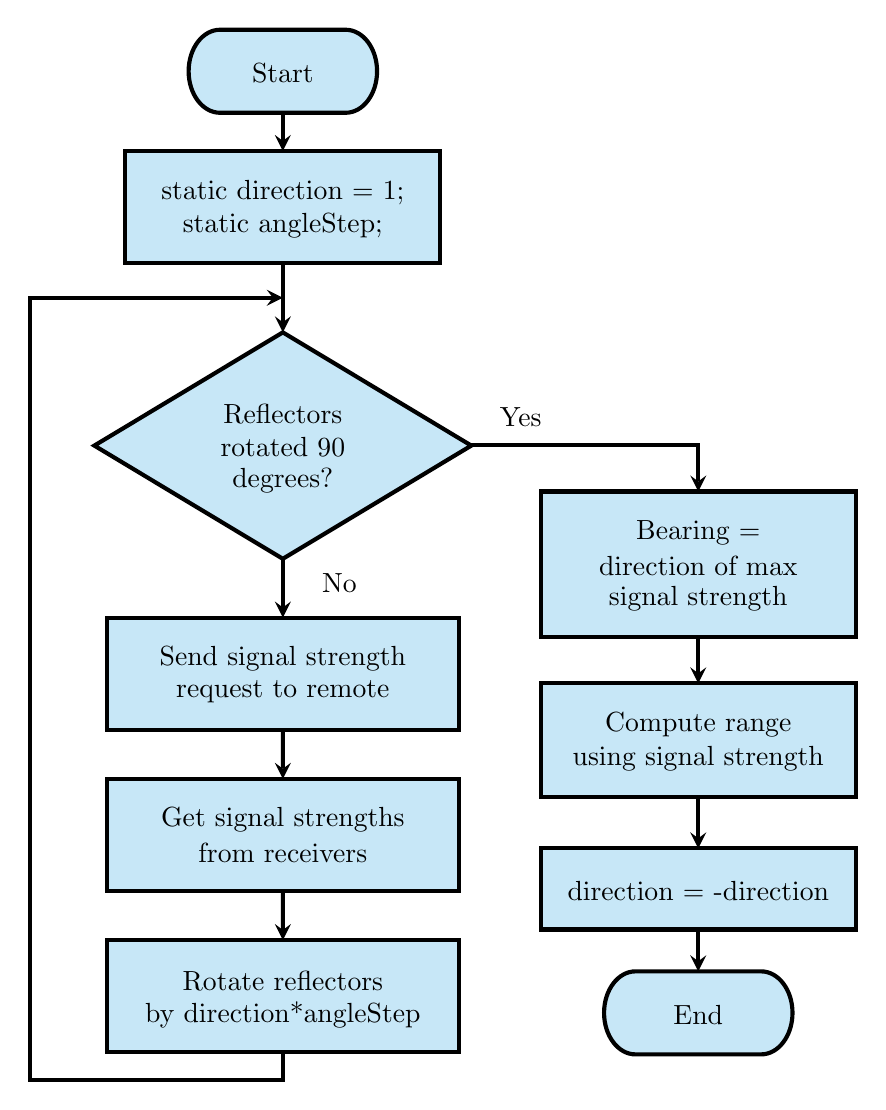
\begin{tikzpicture}
\pgftransformxscale{1.000000}
\pgftransformyscale{-1.000000}
\definecolor{dialinecolor}{rgb}{0.000000, 0.000000, 0.000000}
\pgfsetstrokecolor{dialinecolor}
\definecolor{dialinecolor}{rgb}{1.000000, 1.000000, 1.000000}
\pgfsetfillcolor{dialinecolor}
\pgfsetlinewidth{0.100000\du}
\pgfsetdash{}{0pt}
\pgfsetdash{}{0pt}
\pgfsetbuttcap
\pgfsetmiterjoin
\pgfsetlinewidth{0.100000\du}
\pgfsetbuttcap
\pgfsetmiterjoin
\pgfsetdash{}{0pt}
\definecolor{dialinecolor}{rgb}{0.780392, 0.905882, 0.968627}
\pgfsetfillcolor{dialinecolor}
\pgfpathmoveto{\pgfpoint{23.245563\du}{0.476720\du}}
\pgfpathlineto{\pgfpoint{26.271813\du}{0.476720\du}}
\pgfpathcurveto{\pgfpoint{26.689651\du}{0.476720\du}}{\pgfpoint{27.028375\du}{0.924435\du}}{\pgfpoint{27.028375\du}{1.476720\du}}
\pgfpathcurveto{\pgfpoint{27.028375\du}{2.029005\du}}{\pgfpoint{26.689651\du}{2.476720\du}}{\pgfpoint{26.271813\du}{2.476720\du}}
\pgfpathlineto{\pgfpoint{23.245563\du}{2.476720\du}}
\pgfpathcurveto{\pgfpoint{22.827724\du}{2.476720\du}}{\pgfpoint{22.489000\du}{2.029005\du}}{\pgfpoint{22.489000\du}{1.476720\du}}
\pgfpathcurveto{\pgfpoint{22.489000\du}{0.924435\du}}{\pgfpoint{22.827724\du}{0.476720\du}}{\pgfpoint{23.245563\du}{0.476720\du}}
\pgfusepath{fill}
\definecolor{dialinecolor}{rgb}{0.000000, 0.000000, 0.000000}
\pgfsetstrokecolor{dialinecolor}
\pgfpathmoveto{\pgfpoint{23.245563\du}{0.476720\du}}
\pgfpathlineto{\pgfpoint{26.271813\du}{0.476720\du}}
\pgfpathcurveto{\pgfpoint{26.689651\du}{0.476720\du}}{\pgfpoint{27.028375\du}{0.924435\du}}{\pgfpoint{27.028375\du}{1.476720\du}}
\pgfpathcurveto{\pgfpoint{27.028375\du}{2.029005\du}}{\pgfpoint{26.689651\du}{2.476720\du}}{\pgfpoint{26.271813\du}{2.476720\du}}
\pgfpathlineto{\pgfpoint{23.245563\du}{2.476720\du}}
\pgfpathcurveto{\pgfpoint{22.827724\du}{2.476720\du}}{\pgfpoint{22.489000\du}{2.029005\du}}{\pgfpoint{22.489000\du}{1.476720\du}}
\pgfpathcurveto{\pgfpoint{22.489000\du}{0.924435\du}}{\pgfpoint{22.827724\du}{0.476720\du}}{\pgfpoint{23.245563\du}{0.476720\du}}
\pgfusepath{stroke}
% setfont left to latex
\definecolor{dialinecolor}{rgb}{0.000000, 0.000000, 0.000000}
\pgfsetstrokecolor{dialinecolor}
\node at (24.758688\du,1.516720\du){Start};
\pgfsetlinewidth{0.100000\du}
\pgfsetdash{}{0pt}
\pgfsetdash{}{0pt}
\pgfsetbuttcap
{
\definecolor{dialinecolor}{rgb}{0.000000, 0.000000, 0.000000}
\pgfsetfillcolor{dialinecolor}
% was here!!!
\pgfsetarrowsend{stealth}
\definecolor{dialinecolor}{rgb}{0.000000, 0.000000, 0.000000}
\pgfsetstrokecolor{dialinecolor}
\draw (24.758700\du,13.254900\du)--(24.758700\du,14.638000\du);
}
\pgfsetlinewidth{0.100000\du}
\pgfsetdash{}{0pt}
\pgfsetdash{}{0pt}
\pgfsetbuttcap
{
\definecolor{dialinecolor}{rgb}{0.000000, 0.000000, 0.000000}
\pgfsetfillcolor{dialinecolor}
% was here!!!
\pgfsetarrowsend{stealth}
\definecolor{dialinecolor}{rgb}{0.000000, 0.000000, 0.000000}
\pgfsetstrokecolor{dialinecolor}
\draw (24.758700\du,6.097900\du)--(24.758700\du,7.767000\du);
}
\pgfsetlinewidth{0.100000\du}
\pgfsetdash{}{0pt}
\pgfsetdash{}{0pt}
\pgfsetmiterjoin
\pgfsetbuttcap
{
\definecolor{dialinecolor}{rgb}{0.000000, 0.000000, 0.000000}
\pgfsetfillcolor{dialinecolor}
% was here!!!
\pgfsetarrowsend{stealth}
{\pgfsetcornersarced{\pgfpoint{0.000000\du}{0.000000\du}}\definecolor{dialinecolor}{rgb}{0.000000, 0.000000, 0.000000}
\pgfsetstrokecolor{dialinecolor}
\draw (24.758700\du,25.106700\du)--(24.758700\du,25.775000\du)--(18.662000\du,25.775000\du)--(18.662000\du,6.932450\du)--(24.758700\du,6.932450\du);
}}
\pgfsetlinewidth{0.100000\du}
\pgfsetdash{}{0pt}
\pgfsetdash{}{0pt}
\pgfsetmiterjoin
\pgfsetbuttcap
{
\definecolor{dialinecolor}{rgb}{0.000000, 0.000000, 0.000000}
\pgfsetfillcolor{dialinecolor}
% was here!!!
\pgfsetarrowsend{stealth}
{\pgfsetcornersarced{\pgfpoint{0.000000\du}{0.000000\du}}\definecolor{dialinecolor}{rgb}{0.000000, 0.000000, 0.000000}
\pgfsetstrokecolor{dialinecolor}
\draw (29.260600\du,10.511000\du)--(29.260600\du,10.475000\du)--(34.766550\du,10.475000\du)--(34.766550\du,11.601800\du);
}}
% setfont left to latex
\definecolor{dialinecolor}{rgb}{0.000000, 0.000000, 0.000000}
\pgfsetstrokecolor{dialinecolor}
\node[anchor=west] at (29.716400\du,9.806400\du){Yes};
% setfont left to latex
\definecolor{dialinecolor}{rgb}{0.000000, 0.000000, 0.000000}
\pgfsetstrokecolor{dialinecolor}
\node[anchor=west] at (25.433800\du,13.804600\du){No};
\definecolor{dialinecolor}{rgb}{0.780392, 0.905882, 0.968627}
\pgfsetfillcolor{dialinecolor}
\fill (20.519100\du,18.522300\du)--(20.519100\du,21.222300\du)--(28.998168\du,21.222300\du)--(28.998168\du,18.522300\du)--cycle;
\pgfsetlinewidth{0.100000\du}
\pgfsetdash{}{0pt}
\pgfsetdash{}{0pt}
\pgfsetmiterjoin
\definecolor{dialinecolor}{rgb}{0.000000, 0.000000, 0.000000}
\pgfsetstrokecolor{dialinecolor}
\draw (20.519100\du,18.522300\du)--(20.519100\du,21.222300\du)--(28.998168\du,21.222300\du)--(28.998168\du,18.522300\du)--cycle;
% setfont left to latex
\definecolor{dialinecolor}{rgb}{0.000000, 0.000000, 0.000000}
\pgfsetstrokecolor{dialinecolor}
\node at (24.758634\du,19.512300\du){Get signal strengths};
% setfont left to latex
\definecolor{dialinecolor}{rgb}{0.000000, 0.000000, 0.000000}
\pgfsetstrokecolor{dialinecolor}
\node at (24.758634\du,20.312300\du){from receivers};
\definecolor{dialinecolor}{rgb}{0.780392, 0.905882, 0.968627}
\pgfsetfillcolor{dialinecolor}
\fill (24.758657\du,7.767000\du)--(29.299515\du,10.494357\du)--(24.758657\du,13.221713\du)--(20.217800\du,10.494357\du)--cycle;
\pgfsetlinewidth{0.100000\du}
\pgfsetdash{}{0pt}
\pgfsetdash{}{0pt}
\pgfsetmiterjoin
\definecolor{dialinecolor}{rgb}{0.000000, 0.000000, 0.000000}
\pgfsetstrokecolor{dialinecolor}
\draw (24.758657\du,7.767000\du)--(29.299515\du,10.494357\du)--(24.758657\du,13.221713\du)--(20.217800\du,10.494357\du)--cycle;
% setfont left to latex
\definecolor{dialinecolor}{rgb}{0.000000, 0.000000, 0.000000}
\pgfsetstrokecolor{dialinecolor}
\node at (24.758657\du,9.734357\du){Reflectors};
% setfont left to latex
\definecolor{dialinecolor}{rgb}{0.000000, 0.000000, 0.000000}
\pgfsetstrokecolor{dialinecolor}
\node at (24.758657\du,10.534357\du){rotated 90};
% setfont left to latex
\definecolor{dialinecolor}{rgb}{0.000000, 0.000000, 0.000000}
\pgfsetstrokecolor{dialinecolor}
\node at (24.758657\du,11.334357\du){degrees?};
\definecolor{dialinecolor}{rgb}{0.780392, 0.905882, 0.968627}
\pgfsetfillcolor{dialinecolor}
\fill (30.974050\du,11.601800\du)--(30.974050\du,15.101800\du)--(38.559050\du,15.101800\du)--(38.559050\du,11.601800\du)--cycle;
\pgfsetlinewidth{0.100000\du}
\pgfsetdash{}{0pt}
\pgfsetdash{}{0pt}
\pgfsetmiterjoin
\definecolor{dialinecolor}{rgb}{0.000000, 0.000000, 0.000000}
\pgfsetstrokecolor{dialinecolor}
\draw (30.974050\du,11.601800\du)--(30.974050\du,15.101800\du)--(38.559050\du,15.101800\du)--(38.559050\du,11.601800\du)--cycle;
% setfont left to latex
\definecolor{dialinecolor}{rgb}{0.000000, 0.000000, 0.000000}
\pgfsetstrokecolor{dialinecolor}
\node at (34.766550\du,12.591800\du){Bearing =};
% setfont left to latex
\definecolor{dialinecolor}{rgb}{0.000000, 0.000000, 0.000000}
\pgfsetstrokecolor{dialinecolor}
\node at (34.766550\du,13.391800\du){direction of max};
% setfont left to latex
\definecolor{dialinecolor}{rgb}{0.000000, 0.000000, 0.000000}
\pgfsetstrokecolor{dialinecolor}
\node at (34.766550\du,14.191800\du){signal strength};
\definecolor{dialinecolor}{rgb}{0.780392, 0.905882, 0.968627}
\pgfsetfillcolor{dialinecolor}
\fill (30.974050\du,16.222900\du)--(30.974050\du,18.950000\du)--(38.559050\du,18.950000\du)--(38.559050\du,16.222900\du)--cycle;
\pgfsetlinewidth{0.100000\du}
\pgfsetdash{}{0pt}
\pgfsetdash{}{0pt}
\pgfsetmiterjoin
\definecolor{dialinecolor}{rgb}{0.000000, 0.000000, 0.000000}
\pgfsetstrokecolor{dialinecolor}
\draw (30.974050\du,16.222900\du)--(30.974050\du,18.950000\du)--(38.559050\du,18.950000\du)--(38.559050\du,16.222900\du)--cycle;
% setfont left to latex
\definecolor{dialinecolor}{rgb}{0.000000, 0.000000, 0.000000}
\pgfsetstrokecolor{dialinecolor}
\node at (34.766550\du,17.226450\du){Compute range};
% setfont left to latex
\definecolor{dialinecolor}{rgb}{0.000000, 0.000000, 0.000000}
\pgfsetstrokecolor{dialinecolor}
\node at (34.766550\du,18.026450\du){using signal strength};
\pgfsetlinewidth{0.100000\du}
\pgfsetdash{}{0pt}
\pgfsetdash{}{0pt}
\pgfsetbuttcap
{
\definecolor{dialinecolor}{rgb}{0.000000, 0.000000, 0.000000}
\pgfsetfillcolor{dialinecolor}
% was here!!!
\pgfsetarrowsend{stealth}
\definecolor{dialinecolor}{rgb}{0.000000, 0.000000, 0.000000}
\pgfsetstrokecolor{dialinecolor}
\draw (24.758700\du,17.338000\du)--(24.758600\du,18.522300\du);
}
\pgfsetlinewidth{0.100000\du}
\pgfsetdash{}{0pt}
\pgfsetdash{}{0pt}
\pgfsetbuttcap
{
\definecolor{dialinecolor}{rgb}{0.000000, 0.000000, 0.000000}
\pgfsetfillcolor{dialinecolor}
% was here!!!
\pgfsetarrowsend{stealth}
\definecolor{dialinecolor}{rgb}{0.000000, 0.000000, 0.000000}
\pgfsetstrokecolor{dialinecolor}
\draw (24.758600\du,21.222300\du)--(24.758700\du,22.406700\du);
}
\pgfsetlinewidth{0.100000\du}
\pgfsetdash{}{0pt}
\pgfsetdash{}{0pt}
\pgfsetbuttcap
{
\definecolor{dialinecolor}{rgb}{0.000000, 0.000000, 0.000000}
\pgfsetfillcolor{dialinecolor}
% was here!!!
\pgfsetarrowsend{stealth}
\definecolor{dialinecolor}{rgb}{0.000000, 0.000000, 0.000000}
\pgfsetstrokecolor{dialinecolor}
\draw (34.766550\du,15.101800\du)--(34.766550\du,16.222900\du);
}
\pgfsetlinewidth{0.100000\du}
\pgfsetdash{}{0pt}
\pgfsetdash{}{0pt}
\pgfsetbuttcap
{
\definecolor{dialinecolor}{rgb}{0.000000, 0.000000, 0.000000}
\pgfsetfillcolor{dialinecolor}
% was here!!!
\pgfsetarrowsend{stealth}
\definecolor{dialinecolor}{rgb}{0.000000, 0.000000, 0.000000}
\pgfsetstrokecolor{dialinecolor}
\draw (34.766550\du,18.950000\du)--(34.766550\du,20.197900\du);
}
\definecolor{dialinecolor}{rgb}{0.780392, 0.905882, 0.968627}
\pgfsetfillcolor{dialinecolor}
\fill (20.519100\du,14.638000\du)--(20.519100\du,17.338000\du)--(28.998168\du,17.338000\du)--(28.998168\du,14.638000\du)--cycle;
\pgfsetlinewidth{0.100000\du}
\pgfsetdash{}{0pt}
\pgfsetdash{}{0pt}
\pgfsetmiterjoin
\definecolor{dialinecolor}{rgb}{0.000000, 0.000000, 0.000000}
\pgfsetstrokecolor{dialinecolor}
\draw (20.519100\du,14.638000\du)--(20.519100\du,17.338000\du)--(28.998168\du,17.338000\du)--(28.998168\du,14.638000\du)--cycle;
% setfont left to latex
\definecolor{dialinecolor}{rgb}{0.000000, 0.000000, 0.000000}
\pgfsetstrokecolor{dialinecolor}
\node at (24.758634\du,15.628000\du){Send signal strength};
% setfont left to latex
\definecolor{dialinecolor}{rgb}{0.000000, 0.000000, 0.000000}
\pgfsetstrokecolor{dialinecolor}
\node at (24.758634\du,16.428000\du){request to remote};
\definecolor{dialinecolor}{rgb}{0.780392, 0.905882, 0.968627}
\pgfsetfillcolor{dialinecolor}
\fill (20.519100\du,22.406700\du)--(20.519100\du,25.106700\du)--(28.998168\du,25.106700\du)--(28.998168\du,22.406700\du)--cycle;
\pgfsetlinewidth{0.100000\du}
\pgfsetdash{}{0pt}
\pgfsetdash{}{0pt}
\pgfsetmiterjoin
\definecolor{dialinecolor}{rgb}{0.000000, 0.000000, 0.000000}
\pgfsetstrokecolor{dialinecolor}
\draw (20.519100\du,22.406700\du)--(20.519100\du,25.106700\du)--(28.998168\du,25.106700\du)--(28.998168\du,22.406700\du)--cycle;
% setfont left to latex
\definecolor{dialinecolor}{rgb}{0.000000, 0.000000, 0.000000}
\pgfsetstrokecolor{dialinecolor}
\node at (24.758634\du,23.396700\du){Rotate reflectors};
% setfont left to latex
\definecolor{dialinecolor}{rgb}{0.000000, 0.000000, 0.000000}
\pgfsetstrokecolor{dialinecolor}
\node at (24.758634\du,24.196700\du){by direction*angleStep};
\pgfsetlinewidth{0.100000\du}
\pgfsetdash{}{0pt}
\pgfsetdash{}{0pt}
\pgfsetbuttcap
\pgfsetmiterjoin
\pgfsetlinewidth{0.100000\du}
\pgfsetbuttcap
\pgfsetmiterjoin
\pgfsetdash{}{0pt}
\definecolor{dialinecolor}{rgb}{0.780392, 0.905882, 0.968627}
\pgfsetfillcolor{dialinecolor}
\pgfpathmoveto{\pgfpoint{33.253425\du}{23.159900\du}}
\pgfpathlineto{\pgfpoint{36.279675\du}{23.159900\du}}
\pgfpathcurveto{\pgfpoint{36.697513\du}{23.159900\du}}{\pgfpoint{37.036238\du}{23.607615\du}}{\pgfpoint{37.036238\du}{24.159900\du}}
\pgfpathcurveto{\pgfpoint{37.036238\du}{24.712185\du}}{\pgfpoint{36.697513\du}{25.159900\du}}{\pgfpoint{36.279675\du}{25.159900\du}}
\pgfpathlineto{\pgfpoint{33.253425\du}{25.159900\du}}
\pgfpathcurveto{\pgfpoint{32.835587\du}{25.159900\du}}{\pgfpoint{32.496863\du}{24.712185\du}}{\pgfpoint{32.496863\du}{24.159900\du}}
\pgfpathcurveto{\pgfpoint{32.496863\du}{23.607615\du}}{\pgfpoint{32.835587\du}{23.159900\du}}{\pgfpoint{33.253425\du}{23.159900\du}}
\pgfusepath{fill}
\definecolor{dialinecolor}{rgb}{0.000000, 0.000000, 0.000000}
\pgfsetstrokecolor{dialinecolor}
\pgfpathmoveto{\pgfpoint{33.253425\du}{23.159900\du}}
\pgfpathlineto{\pgfpoint{36.279675\du}{23.159900\du}}
\pgfpathcurveto{\pgfpoint{36.697513\du}{23.159900\du}}{\pgfpoint{37.036238\du}{23.607615\du}}{\pgfpoint{37.036238\du}{24.159900\du}}
\pgfpathcurveto{\pgfpoint{37.036238\du}{24.712185\du}}{\pgfpoint{36.697513\du}{25.159900\du}}{\pgfpoint{36.279675\du}{25.159900\du}}
\pgfpathlineto{\pgfpoint{33.253425\du}{25.159900\du}}
\pgfpathcurveto{\pgfpoint{32.835587\du}{25.159900\du}}{\pgfpoint{32.496863\du}{24.712185\du}}{\pgfpoint{32.496863\du}{24.159900\du}}
\pgfpathcurveto{\pgfpoint{32.496863\du}{23.607615\du}}{\pgfpoint{32.835587\du}{23.159900\du}}{\pgfpoint{33.253425\du}{23.159900\du}}
\pgfusepath{stroke}
% setfont left to latex
\definecolor{dialinecolor}{rgb}{0.000000, 0.000000, 0.000000}
\pgfsetstrokecolor{dialinecolor}
\node at (34.766550\du,24.199900\du){End};
\definecolor{dialinecolor}{rgb}{0.780392, 0.905882, 0.968627}
\pgfsetfillcolor{dialinecolor}
\fill (20.966200\du,3.397900\du)--(20.966200\du,6.097900\du)--(28.551200\du,6.097900\du)--(28.551200\du,3.397900\du)--cycle;
\pgfsetlinewidth{0.100000\du}
\pgfsetdash{}{0pt}
\pgfsetdash{}{0pt}
\pgfsetmiterjoin
\definecolor{dialinecolor}{rgb}{0.000000, 0.000000, 0.000000}
\pgfsetstrokecolor{dialinecolor}
\draw (20.966200\du,3.397900\du)--(20.966200\du,6.097900\du)--(28.551200\du,6.097900\du)--(28.551200\du,3.397900\du)--cycle;
% setfont left to latex
\definecolor{dialinecolor}{rgb}{0.000000, 0.000000, 0.000000}
\pgfsetstrokecolor{dialinecolor}
\node at (24.758700\du,4.387900\du){static direction = 1;};
% setfont left to latex
\definecolor{dialinecolor}{rgb}{0.000000, 0.000000, 0.000000}
\pgfsetstrokecolor{dialinecolor}
\node at (24.758700\du,5.187900\du){static angleStep;};
\pgfsetlinewidth{0.100000\du}
\pgfsetdash{}{0pt}
\pgfsetdash{}{0pt}
\pgfsetbuttcap
{
\definecolor{dialinecolor}{rgb}{0.000000, 0.000000, 0.000000}
\pgfsetfillcolor{dialinecolor}
% was here!!!
\pgfsetarrowsend{stealth}
\definecolor{dialinecolor}{rgb}{0.000000, 0.000000, 0.000000}
\pgfsetstrokecolor{dialinecolor}
\draw (24.758700\du,2.476720\du)--(24.758700\du,3.397900\du);
}
\definecolor{dialinecolor}{rgb}{0.780392, 0.905882, 0.968627}
\pgfsetfillcolor{dialinecolor}
\fill (30.974050\du,20.197900\du)--(30.974050\du,22.150000\du)--(38.559050\du,22.150000\du)--(38.559050\du,20.197900\du)--cycle;
\pgfsetlinewidth{0.100000\du}
\pgfsetdash{}{0pt}
\pgfsetdash{}{0pt}
\pgfsetmiterjoin
\definecolor{dialinecolor}{rgb}{0.000000, 0.000000, 0.000000}
\pgfsetstrokecolor{dialinecolor}
\draw (30.974050\du,20.197900\du)--(30.974050\du,22.150000\du)--(38.559050\du,22.150000\du)--(38.559050\du,20.197900\du)--cycle;
% setfont left to latex
\definecolor{dialinecolor}{rgb}{0.000000, 0.000000, 0.000000}
\pgfsetstrokecolor{dialinecolor}
\node at (34.766550\du,21.213950\du){direction = -direction};
\pgfsetlinewidth{0.100000\du}
\pgfsetdash{}{0pt}
\pgfsetdash{}{0pt}
\pgfsetbuttcap
{
\definecolor{dialinecolor}{rgb}{0.000000, 0.000000, 0.000000}
\pgfsetfillcolor{dialinecolor}
% was here!!!
\pgfsetarrowsend{stealth}
\definecolor{dialinecolor}{rgb}{0.000000, 0.000000, 0.000000}
\pgfsetstrokecolor{dialinecolor}
\draw (34.766550\du,22.150000\du)--(34.766550\du,23.159900\du);
}
\end{tikzpicture}
